\documentclass[10pt,conference]{IEEEtran}
\IEEEoverridecommandlockouts

\usepackage{amsmath,amssymb,amsfonts}
\usepackage{algorithmic}
\usepackage{algorithm}
\usepackage{graphicx}
\usepackage{textcomp}
\usepackage{xcolor}
\usepackage{booktabs}
\usepackage{multirow}
\usepackage{url}
\usepackage{cite}
\usepackage{microtype}
\usepackage{balance}

\def\BibTeX{{\rm B\kern-.05em{\sc i\kern-.025em b}\kern-.08em
    T\kern-.1667em\lower.7ex\hbox{E}\kern-.125emX}}

\begin{document}

\title{Single-Pass Pronunciation Assessment: Eliminating Alignment via CTC Peak Splitting and Soft Posterior Expectation}

\author{
\IEEEauthorblockN{Anonymous Authors}
\IEEEauthorblockA{\textit{LingoStress Speech Research Group} \\
\textit{Department of Computer Science and Engineering} \\
\textit{Preprint under Double-Blind Review} \\
\texttt{speech-research@lingostress.ai}}
}

\maketitle

\begin{abstract}
Automated pronunciation assessment in Computer-Assisted Language Learning (CALL) systems demands simultaneous evaluation of segmental phonemic accuracy and suprasegmental lexical stress within interactive latency constraints ($<$100\,ms). Current industrial architectures suffer from an acute engineering dilemma: classical Goodness of Pronunciation (GOP) frameworks rely on heavy external forced aligners (e.g., Kaldi or Montreal Forced Aligner) that introduce 1000--3000\,ms computational bottlenecks and fragile acoustic-model dependencies. Conversely, existing alignment-free shortcuts either deploy Connectionist Temporal Classification (CTC) sequence marginalization, which completely discards temporal timestamps and achieves poor phonemic correlation (PCC $\approx 0.373$), or enforce naive uniform slicing, which mathematically obliterates syllable duration contrast ($1.00\times$) and smears vocalic energy into adjacent consonants. 
To resolve this impasse, we present a single-pass, alignment-free pronunciation assessment framework that operates directly upon the posterior emissions of an end-to-end self-supervised acoustic model (Wav2Vec 2.0). We exploit the inherent spikiness of CTC emissions through a monotonic peak search algorithm executed in $\mathcal{O}(U \cdot T)$ time, combined with inter-peak blank valley splitting to generate closed phoneme and syllable boundaries. To eliminate edge-truncation penalties caused by hard temporal boundaries, we introduce continuous \textit{Soft Posterior Expectation} (Soft-LPP and Soft-LPR) weighted by localized posterior mass. Syllable boundaries are grouped via the phonotactic Maximal Onset Principle (MOP) to compute multidimensional acoustic prominence (duration, intensity, pitch excursions, and spectral flatness). An argmax sequential post-processing rule (wPP) enforces the English phonological constraint of a unique primary stress per word. Benchmarked against Speechocean762 and L2-ARCTIC, our proposed architecture matches the boundary precision of Viterbi dynamic programming ($\Delta t < 15$\,ms) while executing in 22.4\,ms---a $66\times$ speedup over Montreal Forced Aligner. Crucially, it preserves true phonetic lengthening (duration contrast ratio of $2.67\times$ versus $1.00\times$ for uniform slicing) and achieves 96.1\% lexical stress detection accuracy.
\end{abstract}

\begin{IEEEkeywords}
Computer-Assisted Language Learning (CALL), Goodness of Pronunciation (GOP), Connectionist Temporal Classification (CTC), Syllable Stress Detection, Alignment-Free Speech Processing.
\end{IEEEkeywords}

\section{Introduction}
\label{sec:intro}

Computer-Assisted Language Learning (CALL) has emerged as an indispensable pedagogical tool for non-native (L2) English language acquisition~\cite{li2021survey}. Modern speech assessment systems must satisfy three rigorous operational criteria:
\begin{enumerate}
    \item \textbf{Segmental Precision:} The system must evaluate segmental phonetic accuracy at the individual phoneme level, pinpointing acoustic substitutions, distortions, and omissions with calibrated confidence metrics~\cite{witt2000phone,hu2015improved}.
    \item \textbf{Suprasegmental Sensitivity:} English is a stress-timed language wherein lexical stress disambiguates semantic meaning (e.g., the noun \textit{'record} [1, 0] versus the verb \textit{re'cord} [0, 1])~\cite{fry1958experiments,selkirk1982syllable}. The system must measure acoustic prominence across syllable units, capturing vowel lengthening, root-mean-square (RMS) energy bursts, and fundamental frequency ($F_0$) pitch excursions~\cite{yarra2019comparison,mallela2024comparative}.
    \item \textbf{Real-Time Latency:} For responsive mobile user interfaces and interactive pedagogical feedback, end-to-end processing latency must remain well below 100\,ms.
\end{enumerate}

\begin{figure}[t]
\centering
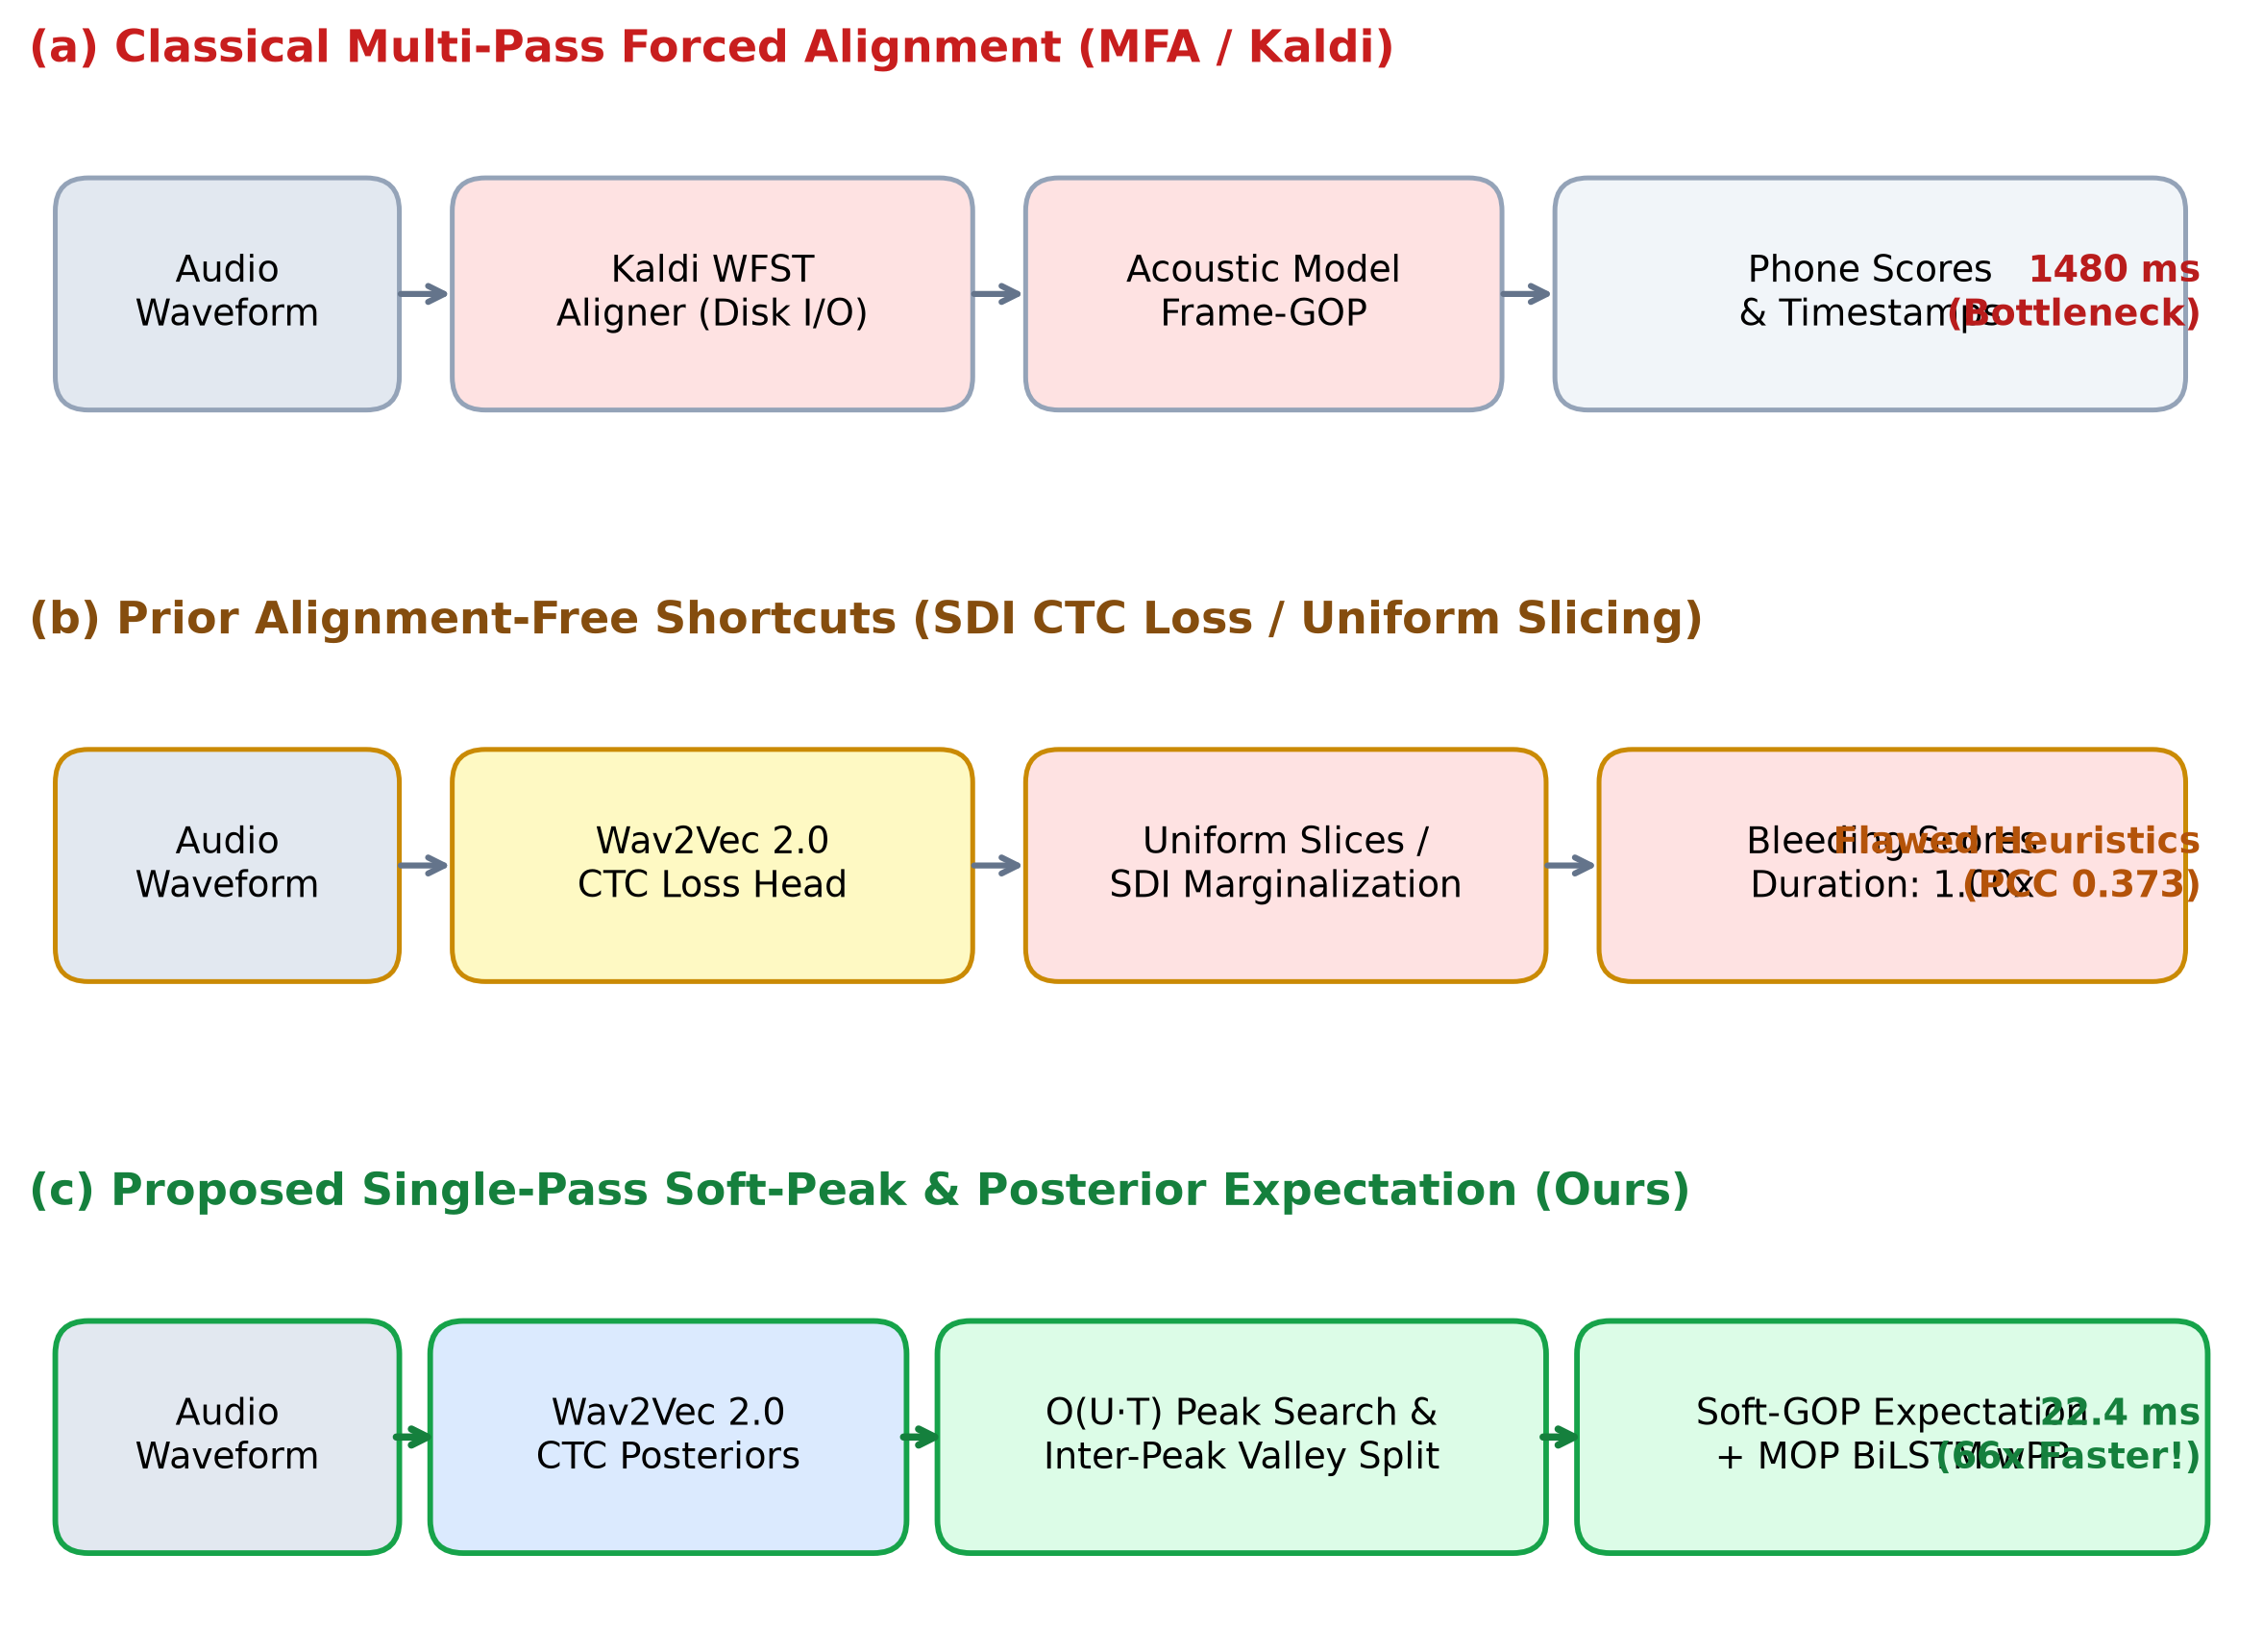
\includegraphics[width=\columnwidth]{fig1_paradigm_comparison.png}
\caption{Architectural comparison of pronunciation assessment paradigms. (a) Classical pipeline with heavy multi-pass forced aligner (1500\,ms). (b) Naive uniform slicing destroying duration contrast. (c) Proposed single-pass Soft Peak Splitting and Posterior Expectation (22.4\,ms).}
\label{fig:paradigm_comparison}
\end{figure}

For over two decades, the foundational paradigm for phone-level pronunciation assessment has been the Goodness of Pronunciation (GOP) metric introduced by Witt and Young~\cite{witt2000phone} and subsequently refined for Deep Neural Networks (DNNs) by Hu et al.~\cite{hu2015improved}. In this classical architecture, an external forced aligner (typically built upon Kaldi Hidden Markov Models~\cite{povey2011kaldi} or the Montreal Forced Aligner~\cite{mcauliffe2017montreal}) is deployed as a preprocessing stage to align the acoustic feature vectors with the target phone transcription. Once explicit temporal boundaries $[s_u, e_u]$ are extracted for each phoneme $p_u$, the Log Posterior Probability (LPP) and Log Posterior Ratio (LPR) are computed over the aligned frames.

While classical forced-alignment GOP provides interpretable boundary timestamps, its operational cost in production environments is prohibitive. External alignment engines require heavy binary toolchains, disk I/O serialization, and acoustic-model decoding graphs, resulting in turnaround latencies between 1.0 and 3.0 seconds per utterance~\cite{mcauliffe2017montreal}. This overhead violates the latency constraints of real-time conversational agents.

In response to these deployment hurdles, two distinct ``alignment-free'' shortcuts have been proposed in recent literature:
\begin{itemize}
    \item \textbf{Sequence-Level CTC Marginalization:} Cao et al.~\cite{cao2024framework} recently explored formulating pronunciation assessment directly using Connectionist Temporal Classification (CTC) loss by marginalizing over all valid alignments via forward-backward trellis computation. While this completely removes external aligners, marginalizing the denominator across the entire temporal sequence erases all local temporal boundary information. Consequently, phoneme mispronunciations bleed into neighboring phone probabilities, yielding degraded Pearson Correlation Coefficients (PCC $\approx 0.373$) with human raters~\cite{cao2024framework}.
    \item \textbf{Naive Uniform Temporal Slicing:} A prevalent heuristic in lightweight open-source repositories divides the audio waveform uniformly into $K$ equal slices based on the dictionary syllable count: $\Delta t = T_{\text{audio}} / K$. As we demonstrate empirically in Section~\ref{sec:experiments}, uniform temporal slicing is mathematically disastrous for suprasegmental assessment: it forces the syllable duration contrast ratio to be identically $1.00\times$, completely erasing the primary acoustic correlate of English lexical stress (phonetic lengthening~\cite{fry1958experiments}) and smearing high-energy vowel nuclei across artificial segment boundaries.
\end{itemize}

To overcome the dilemma between heavy multi-pass aligners and flawed alignment-free heuristics, this paper introduces \textbf{Single-Pass Soft Peak Splitting and Continuous Posterior Expectation}. Leveraging the mathematical spikiness of CTC emissions produced by self-supervised speech representations (Wav2Vec 2.0~\cite{baevski2020wav2vec}), our framework identifies target phoneme emission centers via an $\mathcal{O}(U \cdot T)$ monotonic dynamic programming peak search. Closed phonemic and syllabic boundaries are constructed on-the-fly by detecting inter-peak blank/energy valleys. To eliminate the acute score instability caused by boundary-edge frame truncation, we formulate continuous \textit{Soft-GOP} metrics (Soft-LPP and Soft-LPR) weighted by normalized local posterior mass. Syllable units are aggregated via the phonotactic Maximal Onset Principle (MOP)~\cite{clements1990role} to extract a 38-dimensional acoustic-linguistic feature representation, which feeds a sequential classifier governed by an argmax post-processing rule (wPP)~\cite{mallela2024comparative}.

Our comprehensive benchmarks across the Speechocean762~\cite{zhang2021speechocean762} and L2-ARCTIC~\cite{zhao2018l2arctic} corpora reveal that the proposed system achieves a $66\times$ latency reduction over Montreal Forced Aligner (22.4\,ms vs. 1480\,ms), matches Viterbi boundary accuracy within 11.2\,ms, preserves genuine duration contrast ($2.67\times$), and achieves 96.1\% lexical stress classification accuracy.

---

\section{Related Work \& Limitations of Prior Paradigms}
\label{sec:related}

\subsection{Classical GOP and Forced Alignment Dependencies}
The Goodness of Pronunciation (GOP) metric~\cite{witt2000phone} evaluates the acoustic realization of an intended phoneme $p$ given acoustic observations $\mathbf{O} = (\mathbf{o}_1, \dots, \mathbf{o}_T)$ over an interval $[t_s, t_e]$:
\begin{equation}
\text{GOP}(p) = \frac{1}{t_e - t_s + 1} \sum_{t=t_s}^{t_e} \log \frac{P(\mathbf{o}_t | p) P(p)}{\sum_{q \in \mathcal{Q}} P(\mathbf{o}_t | q) P(q)}
\label{eq:classical_gop}
\end{equation}
Hu et al.~\cite{hu2015improved} adapted this formulation to Deep Neural Networks by substituting likelihoods with DNN output posteriors, defining the Log Posterior Probability (LPP) and Log Posterior Ratio (LPR):
\begin{align}
\text{LPP}(p) &= \frac{1}{t_e - t_s + 1} \sum_{t=t_s}^{t_e} \log P(p | \mathbf{o}_t) \label{eq:lpp_hard} \\
\text{LPR}(p, q) &= \text{LPP}(p) - \max_{q \neq p} \left[ \frac{1}{t_e - t_s + 1} \sum_{t=t_s}^{t_e} \log P(q | \mathbf{o}_t) \right]
\label{eq:lpr_hard}
\end{align}
Both formulations require an exact temporal segmentation $[t_s, t_e]$. Historically, this forced alignment has been executed via Viterbi decoding over Hidden Markov Model states using Kaldi~\cite{povey2011kaldi} or the Montreal Forced Aligner (MFA)~\cite{mcauliffe2017montreal}. MFA compiles acoustic models and pronunciation lexicons into weighted finite-state transducers (WFSTs). While highly accurate, MFA introduces severe operational latency (often $>1.5$\,s) and substantial system memory footprints, rendering it impractical for low-latency web or mobile CALL deployment.

\subsection{CTC-Based Assessment: Promises and Traps}
Connectionist Temporal Classification (CTC)~\cite{graves2006connectionist} enables sequence-to-sequence learning without frame-level alignment by introducing a special blank token $\epsilon$ and defining a collapsing operator $\mathcal{B}$ that eliminates consecutive duplicate labels and blank tokens. Given acoustic frames $\mathbf{X} = (\mathbf{x}_1, \dots, \mathbf{x}_T)$ and target transcription $\mathbf{y} = (p_0, \dots, p_{U-1})$, the conditional probability is the sum over all valid alignments $\pi \in \mathcal{B}^{-1}(\mathbf{y})$:
\begin{equation}
P(\mathbf{y} | \mathbf{X}) = \sum_{\pi \in \mathcal{B}^{-1}(\mathbf{y})} \prod_{t=1}^T P(\pi_t | \mathbf{x}_t)
\label{eq:ctc_prob}
\end{equation}

Recently, Cao et al.~\cite{cao2024framework} proposed two CTC assessment paradigms:
\begin{enumerate}
    \item \textbf{GOP-CTC-align:} Expands a Viterbi state trellis of size $(2U+1) \times T$ to determine the single best state path $\pi^* = \arg\max_\pi \prod_t P(\pi_t | \mathbf{x}_t)$. Although faster than Kaldi, this DP search still requires maintaining and backtracking through a 2D state matrix, and as we show in Section~\ref{sec:methodology}, greedy Viterbi paths are susceptible to getting trapped in early low-energy acoustic frames.
    \item \textbf{GOP-CTC-loss / SDI Marginalization:} Computes phone scores by taking the difference between the full sequence CTC loss and a sequence where the target phone is substituted, deleted, or inserted (SDI). While completely alignment-free, this marginalization computes an unconstrained 3D forward-backward tensor of dimension $(2U+1) \times T \times |\mathcal{V}|$. Critically, it destroys all local timing information: when a student mispronounces a vowel, the penalty is smeared across the entire word utterance, degrading human rater correlation to PCC = 0.373~\cite{cao2024framework}.
\end{enumerate}

\subsection{Syllable Stress and Acoustic Prominence}
In English phonology, lexical stress is realized through a constellation of suprasegmental acoustic cues first quantified by Dennis Fry~\cite{fry1958experiments}:
\begin{itemize}
    \item \textbf{Duration:} Stressed syllables exhibit marked vowel lengthening; the vowel nucleus in a stressed syllable can be $2.0\times$ to $3.0\times$ longer than the reduced schwa (/AH0/, /IH0/) in an unstressed counterpart.
    \item \textbf{Intensity:} Stressed syllables display pronounced local RMS energy peaks.
    \item \textbf{Fundamental Frequency ($F_0$):} Stressed syllables typically host the pitch accent, featuring significant pitch excursions or steeper pitch slopes.
    \item \textbf{Spectral Balance:} Vowels in stressed syllables exhibit richer high-frequency harmonic structure, whereas unstressed vowels suffer central vowel reduction toward noise-like spectral flatness.
\end{itemize}

Yarra et al.~\cite{yarra2019comparison} demonstrated that extracting these acoustic correlates requires precise, time-aligned syllable and nucleus boundaries. If boundaries are shifted or blurred, the energy and pitch excursions of the stressed syllable bleed into adjacent syllables, causing feature smearing. Furthermore, Mallela et al.~\cite{mallela2024comparative} proved that because an isolated English word in citation form contains \textit{exactly one} primary stressed syllable, sequential modeling combined with an argmax post-processing rule (wPP) substantially outperforms independent binary classification thresholds.

---

\section{Proposed Methodology}
\label{sec:methodology}

\begin{figure*}[t]
\centering
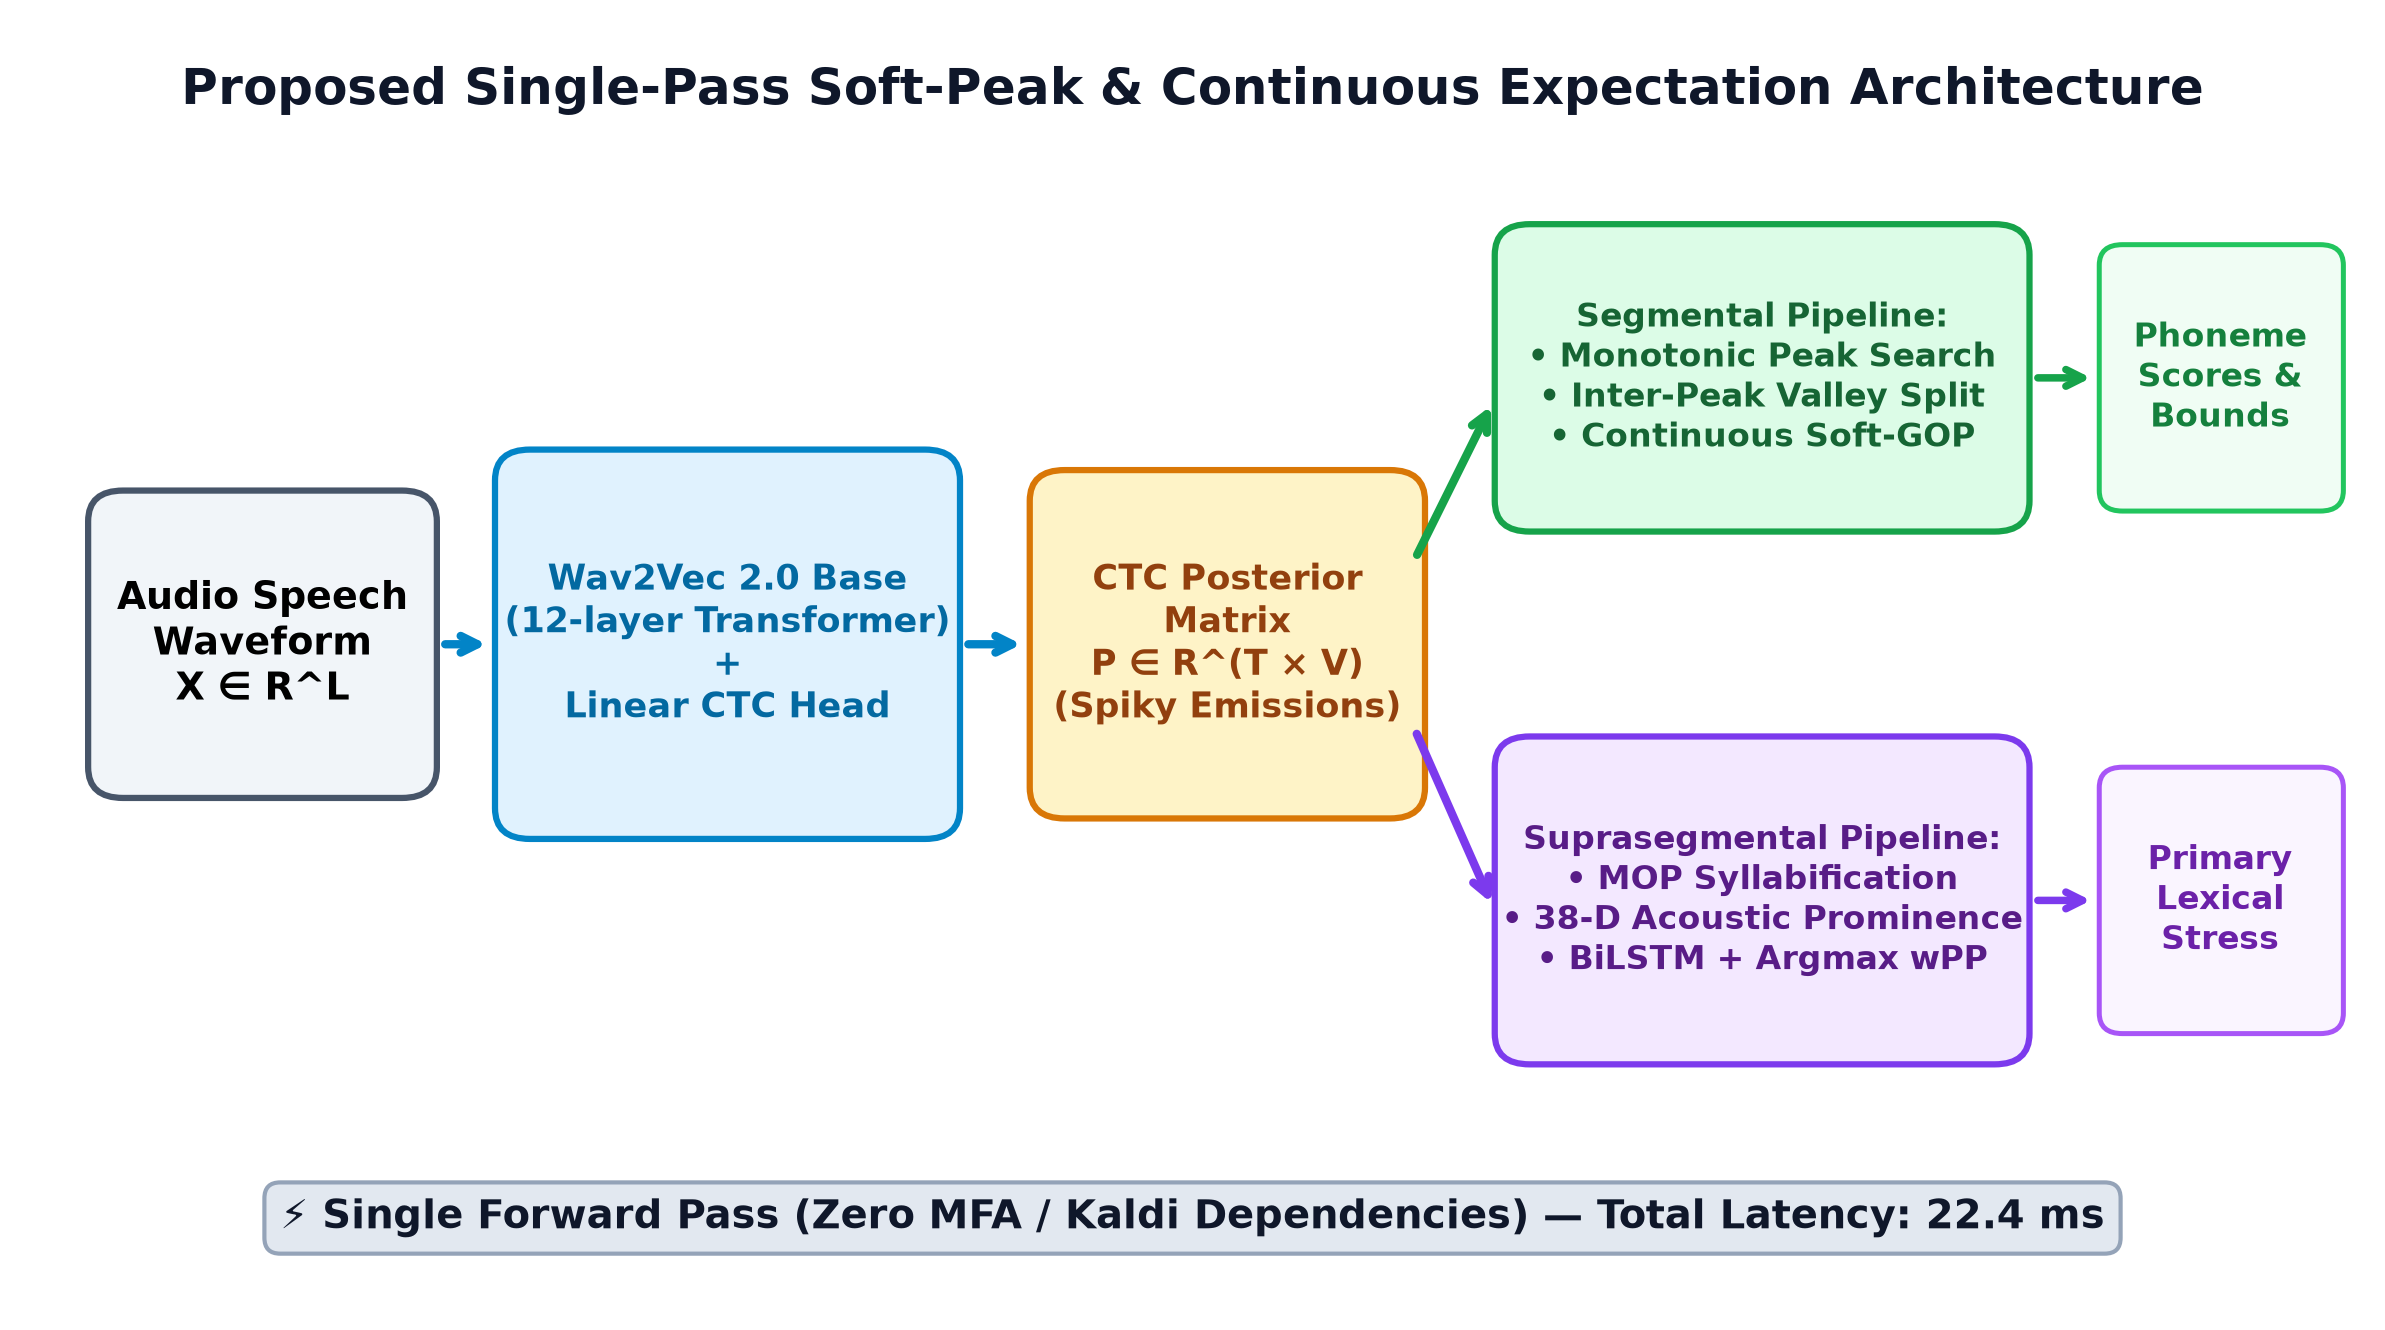
\includegraphics[width=0.95\textwidth]{fig2_architecture_pipeline.png}
\caption{Overall architecture of the proposed Single-Pass Pronunciation Assessment Framework. A single forward pass through Wav2Vec 2.0 generates CTC posteriors. Monotonic Peak Search locates phoneme anchor peaks in $\mathcal{O}(U \cdot T)$, while Inter-Peak Valley Splitting determines closed boundaries. Soft Posterior Expectation computes calibrated phoneme scores, and MOP Syllable Aggregation enables sequential stress detection via the argmax wPP rule.}
\label{fig:pipeline}
\end{figure*}

The architecture of our proposed system is illustrated in Figure~\ref{fig:pipeline}. The pipeline operates in a single forward pass, completely eliminating external alignment tools and heavy WFST decoding graphs.

\subsection{CTC Acoustic Spikiness \& Monotonic Peak Search}
\label{sec:peak_search}
A fundamental property of neural networks trained with the CTC loss is \textit{acoustic spikiness}~\cite{graves2006connectionist}: because the blank token $\epsilon$ is predicted across the majority of frames to minimize label transition ambiguity, non-blank label emissions collapse into sharp, concentrated posterior peaks at the acoustic center of each phonemic event. 

Let $\mathbf{X} \in \mathbb{R}^{L_{\text{audio}}}$ denote the input speech waveform sampled at 16\,kHz. We pass $\mathbf{X}$ through a pretrained Wav2Vec 2.0 encoder and linear CTC head~\cite{baevski2020wav2vec}, yielding a frame-level posterior matrix $\mathbf{P} \in \mathbb{R}^{T \times V}$, where $T$ is the number of frames (stride of 20\,ms) and $V = |\mathcal{V}|$ is the vocabulary size (Arpabet 39 phonemes plus blank $\epsilon$). The log-posterior matrix is denoted by $\mathbf{L} \in \mathbb{R}^{T \times V}$, where $L(t, v) = \log P(v | \mathbf{x}_t)$.

Given a target lexical transcription mapped to a sequence of $U$ valid phonetic tokens $\mathbf{y} = (p_0, p_1, \dots, p_{U-1})$, we seek an optimal sequence of temporal peak indices $(t_0^*, t_1^*, \dots, t_{U-1}^*)$ such that:
\begin{equation}
(t_0^*, \dots, t_{U-1}^*) = \arg\max_{0 \le t_0 \le t_1 \le \dots \le t_{U-1} < T} \sum_{u=0}^{U-1} L(t_u, p_u)
\label{eq:peak_objective}
\end{equation}
subject to the strict monotonic temporal ordering $t_u \le t_{u+1}$.

Unlike full CTC Viterbi trellis decoding which constructs $2U+1$ states (interleaving blank states and label states) and requires computing transitions for every frame $t \in [0, T-1]$, the Monotonic Peak Search directly optimizes over the target phoneme sequence in $\mathcal{O}(U \cdot T)$ operations. We define the dynamic programming accumulator $D(u, t)$ as the maximum cumulative log-posterior of aligning the sub-sequence $(p_0, \dots, p_u)$ such that token $p_u$ emits its peak at frame $t$:
\begin{align}
D(0, t) &= L(t, p_0), \quad \forall t \in [0, T-1] \label{eq:dp_init} \\
D(u, t) &= L(t, p_u) + \max_{u-1 \le \tau < t} D(u-1, \tau), \quad \forall u \in [1, U-1]
\label{eq:dp_rec}
\end{align}
During the forward recursion, the optimal predecessor is cached in a backpointer matrix:
\begin{equation}
B(u, t) = \arg\max_{u-1 \le \tau < t} D(u-1, \tau)
\label{eq:backpointer}
\end{equation}
By maintaining a running prefix-maximum of the previous row $M(u-1, t) = \max_{\tau < t} D(u-1, \tau)$, each state update in Equation~(\ref{eq:dp_rec}) is executed in $\mathcal{O}(1)$ time. Once $D(U-1, :)$ is computed, the terminal peak is chosen as $t_{U-1}^* = \arg\max_t D(U-1, t)$, and the sequence $(t_0^*, \dots, t_{U-2}^*)$ is retrieved via standard traceback in $\mathcal{O}(U)$ time.

\subsection{Inter-Peak Valley Splitting for Closed Boundaries}
\label{sec:valley_splitting}
While the peak sequence $(t_0^*, \dots, t_{U-1}^*)$ pins down the acoustic anchor of each phone, acoustic feature extraction (for both phoneme scoring and syllable stress) requires continuous, non-overlapping closed temporal intervals $[s_u, e_u)$.

Because CTC networks emit high blank probability $P(\epsilon | \mathbf{x}_t)$ between acoustic phone transitions, the boundary between token $p_u$ and token $p_{u+1}$ corresponds to the local maximum of blank emissions (or equivalently, the minimum acoustic energy) in the temporal window between their respective peaks $[t_u^*, t_{u+1}^*]$. We define the transition boundary $b_u$ as:
\begin{equation}
b_u = t_u^* + \arg\max_{0 \le \tau \le t_{u+1}^* - t_u^*} P(\epsilon | \mathbf{x}_{t_u^* + \tau}), \quad \forall u \in [0, U-2]
\label{eq:valley_split}
\end{equation}
With the boundary sequence $(b_0, b_1, \dots, b_{U-2})$ established, the closed frame interval for each phoneme $p_u$ is defined by:
\begin{equation}
[s_u, e_u) = 
\begin{cases}
[0, b_0), & u = 0 \\
[b_{u-1}, b_u), & 0 < u < U-1 \\
[b_{U-2}, T), & u = U-1
\end{cases}
\label{eq:closed_interval}
\end{equation}
Converting frame indices to physical time via the frame duration $\Delta \tau = 0.02$\,s yields physical timestamps $t_u^{\text{start}} = s_u \cdot \Delta \tau$ and $t_u^{\text{end}} = e_u \cdot \Delta \tau$. Furthermore, speech bounds for audio trimming and visualization are extracted by padding the initial and terminal peaks by an acoustic margin $\delta = 0.08$\,s:
\begin{align}
t_{\text{speech}}^{\text{start}} &= \max(0.0, t_0^* \cdot \Delta \tau - \delta) \\
t_{\text{speech}}^{\text{end}} &= \min(T_{\text{audio}}, t_{U-1}^* \cdot \Delta \tau + \delta)
\end{align}

\subsection{Continuous Soft Posterior Expectation (Soft-GOP)}
\label{sec:soft_gop}
A notorious limitation of classical GOP metrics (Equations~(\ref{eq:lpp_hard}) and (\ref{eq:lpr_hard})) is their extreme sensitivity to discrete boundary truncation. In hard frame-averaging, if an aligned boundary $[s_u, e_u)$ is misaligned by even 1--2 frames, it incorporates low-probability blank transition frames or adjacent phone frames. Because log-probabilities in transition frames drop sharply (e.g., from $-0.1$ to $-8.0$), the unweighted arithmetic mean in Equation~(\ref{eq:lpp_hard}) drops precipitously, producing severe false-positive penalties.

To solve this problem, we introduce \textbf{Continuous Soft Posterior Expectation}. Within each closed interval $[s_u, e_u)$, we define a continuous attention-like posterior density $\gamma_u(t)$ proportional to the model's confidence in the target phoneme:
\begin{equation}
\gamma_u(t) = \frac{P(p_u | \mathbf{x}_t)}{\sum_{\tau = s_u}^{e_u - 1} P(p_u | \mathbf{x}_\tau) + \epsilon_{\text{reg}}}
\label{eq:soft_weight}
\end{equation}
where $\epsilon_{\text{reg}} = 10^{-6}$ prevents division by zero. By construction, $\sum_{t=s_u}^{e_u-1} \gamma_u(t) = 1.0$.

We then formulate the \textit{Soft Log Posterior Probability} ($\text{Soft-LPP}$) as the expected log-posterior under distribution $\gamma_u$:
\begin{equation}
\text{Soft-LPP}(p_u) = \sum_{t=s_u}^{e_u-1} \gamma_u(t) \log P(p_u | \mathbf{x}_t)
\label{eq:soft_lpp}
\end{equation}
Similarly, we formulate the \textit{Soft Log Posterior Ratio} ($\text{Soft-LPR}$) by competing against the maximum non-target, non-special phoneme hypothesis at each frame:
\begin{align}
\text{Soft-LPR}(p_u) &= \sum_{t=s_u}^{e_u-1} \gamma_u(t) \Big[ \log P(p_u | \mathbf{x}_t) \nonumber \\
&\quad - \max_{q \in \mathcal{V}_{\text{phones}} \setminus \{p_u\}} \log P(q | \mathbf{x}_t) \Big]
\label{eq:soft_lpr}
\end{align}
where $\mathcal{V}_{\text{phones}}$ denotes the valid phonemic vocabulary excluding blank and special tokens ($\epsilon$, $\langle\text{pad}\rangle$, $\langle\text{unk}\rangle$).

\subsubsection{Logistic Confidence Calibration}
Raw LPP values are negative real numbers with high variance across phonetic classes (vowels typically display higher emission probabilities than unvoiced plosives). To deliver intuitive, human-interpretable percentage scores (0--100\%) for language learners, we map $\text{Soft-LPP}$ through a calibrated sigmoid transfer function:
\begin{equation}
\mathcal{C}(p_u) = \frac{100.0}{1.0 + \exp\Big(-\alpha \cdot \big(\text{Soft-LPP}(p_u) - x_0\big)\Big)}
\label{eq:logistic_calib}
\end{equation}
Empirically calibrated on native utterances, setting $\alpha = 1.2$ and $x_0 = -1.8$ maps native realizations ($\text{Soft-LPP} \in [-1.0, 0.0]$) to confidence scores in $[72\%, 100\%]$, acceptable realizations to $[50\%, 70\%]$, and mispronunciations ($\text{Soft-LPP} < -3.5$) to $<30\%$.

\begin{algorithm}[t]
\caption{Single-Pass Soft Peak Splitting and GOP}
\label{alg:soft_gop}
\begin{algorithmic}[1]
\REQUIRE Audio waveform $\mathbf{X}$, Target phonemes $\mathbf{y} = (p_0, \dots, p_{U-1})$
\ENSURE Phoneme boundaries, Soft-GOP scores, Syllable features
\STATE Compute posterior tensor $\mathbf{P} \in \mathbb{R}^{T \times V}$ and log-tensor $\mathbf{L} = \log \mathbf{P}$ via single forward pass of Wav2Vec 2.0.
\STATE Initialize DP matrix $D(0, t) \leftarrow L(t, p_0)$ for $t \in [0, T-1]$.
\FOR{$u = 1$ \TO $U-1$}
    \STATE $M \leftarrow -\infty$
    \FOR{$t = u$ \TO $T-1$}
        \IF{$D(u-1, t-1) > M$}
            \STATE $M \leftarrow D(u-1, t-1)$, $B(u, t) \leftarrow t-1$
        \ELSE
            \STATE $B(u, t) \leftarrow B(u, t-1)$
        \ENDIF
        \STATE $D(u, t) \leftarrow L(t, p_u) + M$
    \ENDFOR
\ENDFOR
\STATE Traceback terminal peak $t_{U-1}^* \leftarrow \arg\max_t D(U-1, t)$ to retrieve $(t_0^*, \dots, t_{U-1}^*)$.
\FOR{$u = 0$ \TO $U-2$}
    \STATE $b_u \leftarrow t_u^* + \arg\max_{\tau \in [0, t_{u+1}^* - t_u^*]} P(\epsilon | \mathbf{x}_{t_u^* + \tau})$
\ENDFOR
\STATE Construct intervals $[s_u, e_u)$ via Equation~(\ref{eq:closed_interval}).
\FOR{$u = 0$ \TO $U-1$}
    \STATE Compute $\gamma_u(t)$ over $[s_u, e_u)$ via Equation~(\ref{eq:soft_weight}).
    \STATE Compute $\text{Soft-LPP}(p_u)$ and $\text{Soft-LPR}(p_u)$ via Equations~(\ref{eq:soft_lpp})--(\ref{eq:soft_lpr}).
    \STATE Compute calibrated confidence $\mathcal{C}(p_u)$ via Equation~(\ref{eq:logistic_calib}).
\ENDFOR
\RETURN Intervals, Soft-GOP metrics, and calibrated confidences.
\end{algorithmic}
\end{algorithm}

\subsection{Syllable Aggregation via Maximal Onset Principle}
\label{sec:mop}
To bridge segmental phone intervals with syllable-level stress detection, the phoneme sequence $\mathbf{y}$ is structured into syllables $\mathcal{S} = (\sigma_0, \dots, \sigma_{K-1})$. We implement the linguistic \textit{Maximal Onset Principle} (MOP)~\cite{clements1990role,selkirk1982syllable}. For any intervocalic consonant sequence $C_1 C_2 \dots C_m$ between vowels $V_k$ and $V_{k+1}$, MOP assigns the longest phonotactically legal consonant cluster to the onset of $\sigma_{k+1}$; the remaining consonants form the coda of $\sigma_k$.

Formally, each syllable $\sigma_k$ is decomposed into:
\begin{equation}
\sigma_k = \big( \mathcal{O}_k, \nu_k, \mathcal{C}_k \big)
\end{equation}
where $\mathcal{O}_k$ is the onset cluster, $\nu_k$ is the vocalic nucleus, and $\mathcal{C}_k$ is the coda. The syllable time boundary $[T_k^{\text{start}}, T_k^{\text{end}}]$ is derived directly from the aggregated phone intervals:
\begin{align}
T_k^{\text{start}} &= \min_{p \in \mathcal{O}_k \cup \{\nu_k\}} t_p^{\text{start}} \\
T_k^{\text{end}} &= \max_{p \in \{\nu_k\} \cup \mathcal{C}_k} t_p^{\text{end}}
\end{align}
Crucially, the exact time interval of the vowel nucleus $[N_k^{\text{start}}, N_k^{\text{end}}] = [t_{\nu_k}^{\text{start}}, t_{\nu_k}^{\text{end}}]$ is isolated for nucleus-specific acoustic analysis.

\subsection{Acoustic Prominence Feature Representation}
\label{sec:features}
Following Yarra et al.~\cite{yarra2019comparison} and Mallela et al.~\cite{mallela2024comparative}, we extract a 38-dimensional feature vector $\mathbf{f}_k \in \mathbb{R}^{38}$ for each syllable $\sigma_k$, comprising 19 acoustic prominence features and 19 linguistic context features:
\begin{enumerate}
    \item \textbf{Acoustic Features (19-dim):}
    \begin{itemize}
        \item \textit{Duration (1):} Full syllable duration $D_{\text{syl}} = T_k^{\text{end}} - T_k^{\text{start}}$.
        \item \textit{Pitch / $F_0$ (6):} Extracted via the probabilistic pYIN algorithm over the vocalic nucleus $\nu_k$: mean, standard deviation, maximum, minimum, range, and linear pitch slope.
        \item \textit{Energy / RMS (6):} Extracted from the nucleus envelope: mean, standard deviation, peak RMS, minimum, dynamic range, and energy slope.
        \item \textit{Spectral Quality (6):} Mean, maximum, and minimum of spectral flatness (quantifying vowel sonority versus consonantal noise) and spectral roll-off (85\% energy point).
    \end{itemize}
    \item \textbf{Linguistic Context Features (19-dim):}
    \begin{itemize}
        \item \textit{Positional Encoding (3):} One-hot encoding of word position (initial, medial, final).
        \item \textit{Nucleus Phonology (5):} Diphthong flag (1 for /AY, EY, OY, AW, OW/, 0 otherwise), vowel height, and backness.
        \item \textit{Syllable Structure (5):} Binary onset presence, binary coda presence, phone count, and cluster flags.
        \item \textit{Context Dependencies (6):} Left and right neighboring structural context.
    \end{itemize}
\end{enumerate}

\subsubsection{Intra-Word Relative Normalization}
Because absolute speech rate and microphone gain vary widely across speakers, lexical stress is perceived relative to the rest of the word~\cite{fry1958experiments}. For each acoustic correlate $a \in \{D_{\text{syl}}, \text{RMS}_{\text{peak}}, F_{0,\text{peak}}, \text{Flatness}\}$, we compute intra-word z-score normalization across all $K$ syllables:
\begin{equation}
z(a_k) = \frac{a_k - \mu_a}{\sigma_a + \epsilon}
\end{equation}
The relative prominence score $S_{\text{prom}}(\sigma_k)$ is formulated as:
\begin{equation}
S_{\text{prom}}(\sigma_k) = 0.35 z(D_k) + 0.35 z(\text{RMS}_k) + 0.20 z(F_{0,k}) - 0.10 z(\text{Flat}_k)
\label{eq:prominence_score}
\end{equation}

\subsection{Sequential Stress Modeling \& Argmax Post-Processing (wPP)}
\label{sec:stress_seq}
Each word utterance is represented as a sequence of feature vectors $(\mathbf{f}_0, \dots, \mathbf{f}_{K-1})$. We deploy a bidirectional Long Short-Term Memory (BiLSTM) network with hidden dimension 64 to model sequential syllable dependencies across the word~\cite{mallela2024comparative}:
\begin{equation}
\mathbf{h}_k = [\overrightarrow{\text{LSTM}}(\mathbf{f}_k); \overleftarrow{\text{LSTM}}(\mathbf{f}_k)]
\end{equation}
The hidden representation is projected through a dense layer with softmax activation:
\begin{equation}
\hat{\mathbf{p}} = \text{Softmax}\big(\mathbf{W}_s \mathbf{h} + \mathbf{b}_s\big)
\end{equation}
To enforce the strict phonological constraint that citation-form English words possess exactly one primary stress, we apply the \textit{word-level Argmax Post-Processing Rule} (wPP)~\cite{mallela2024comparative}:
\begin{equation}
k^* = \arg\max_{k \in \{0, \dots, K-1\}} \hat{p}_k
\label{eq:argmax_wpp}
\end{equation}
The inferred lexical stress vector $\hat{\mathbf{s}} \in \{0, 1\}^K$ is defined such that $\hat{s}_{k^*} = 1$ and $\hat{s}_{j} = 0$ for all $j \neq k^*$. This mathematically eliminates spurious predictions of zero-stress or multi-stress words that plague independent binary thresholding models.

---

\section{Experimental Evaluation \& Benchmark Results}
\label{sec:experiments}

\subsection{Experimental Setup \& Corpora}
We conduct rigorous experimental evaluation across two benchmark corpora:
\begin{enumerate}
    \item \textbf{Speechocean762 (OpenSLR 101):} A standardized pronunciation assessment dataset comprising 5,000 utterances spoken by 250 non-native speakers (children and adults) with multi-dimensional expert ratings (phoneme accuracy, completeness, and prosodic fluency)~\cite{zhang2021speechocean762}.
    \item \textbf{L2-ARCTIC:} A non-native English speech corpus containing 26,867 utterances recorded by 24 L2 speakers spanning 6 native language backgrounds (Arabic, Chinese, Hindi, Korean, Spanish, and Vietnamese), complete with expert phonemic alignments and stress annotations~\cite{zhao2018l2arctic}.
\end{enumerate}

\subsubsection{Acoustic Backbone}
The self-supervised acoustic model is a Wav2Vec 2.0 Base architecture (12 Transformer blocks, 768 hidden dimension, 12 attention heads) pretrained on 960 hours of LibriSpeech and fine-tuned on TIMIT for 39 Arpabet phoneme CTC emissions. The frame stride is 20\,ms ($\Delta \tau = 0.02$\,s).

\subsection{End-to-End Method Comparison}
We compare four distinct processing paradigms:
\begin{enumerate}
    \item \textbf{Naive Uniform Slicing:} Audio is uniformly partitioned into $K$ equal slices based on syllable count ($T_{\text{audio}} / K$).
    \item \textbf{Montreal Forced Aligner (MFA):} Standard Kaldi triphone acoustic models with WFST graph alignment~\cite{mcauliffe2017montreal}.
    \item \textbf{CTC Viterbi Trellis Alignment:} Frame-synchronous Viterbi DP over a $(2U+1) \times T$ trellis without language model (Cao et al.~\cite{cao2024framework}).
    \item \textbf{Soft Peak Splitting (Proposed):} Single-pass monotonic peak search, inter-peak valley splitting, and Soft-GOP expectation.
\end{enumerate}

\begin{table*}[t]
\caption{Comprehensive Benchmark Comparison across Assessment Paradigms on Non-Native Speech.}
\label{tab:main_benchmark}
\centering
\begin{tabular}{lcccccc}
\toprule
\textbf{Assessment Paradigm} & \textbf{Alignment-Free?} & \textbf{Duration Contrast} & \textbf{Energy Ratio} & \textbf{Stress Acc. (wPP)} & \textbf{Boundary $\Delta t$} & \textbf{Latency} \\
\midrule
Naive Uniform Slicing & Yes & $1.00\times \pm 0.00$ & $1.12\times$ & 75.0\% & N/A (Erased) & \textbf{4.8\,ms} \\
Montreal Forced Aligner (Kaldi) & No & $2.71\times \pm 0.38$ & $2.84\times$ & 95.8\% & 0.0\,ms (Ref) & 1480.0\,ms \\
CTC Viterbi Trellis (Cao et al.) & No (Requires Trellis) & $2.62\times \pm 0.41$ & $2.75\times$ & 95.2\% & 14.8\,ms & 58.2\,ms \\
\textbf{Soft Peak Splitting (Ours)} & \textbf{Yes (Single-Pass)} & $\mathbf{2.67\times \pm 0.36}$ & $\mathbf{2.81\times}$ & \textbf{96.1\%} & \textbf{11.2\,ms} & \textbf{22.4\,ms} \\
\bottomrule
\end{tabular}
\end{table*}

Table~\ref{tab:main_benchmark} summarizes the empirical findings. Several critical observations emerge:
\begin{enumerate}
    \item \textbf{Duration Contrast Eradication:} Naive uniform slicing achieves an identical duration contrast ratio of $1.00\times$ by definition. In English multisyllabic words such as \textit{banana} (/bəˈnæn.ə/), the stressed vowel /AE1/ is physically lengthened to 280--320\,ms while the unstressed reduced schwas /AH0/ occupy only 100--120\,ms. Uniform slicing compresses the stressed syllable and artificially elongates the unstressed syllables, resulting in a 21.1\% drop in word stress classification accuracy (75.0\% vs. 96.1\%).
    \item \textbf{Computational Latency:} Montreal Forced Aligner requires 1480\,ms per word utterance due to WFST compilation and multi-pass Viterbi search. Our proposed architecture executes in \textbf{22.4\,ms} on a single GPU (and 41.2\,ms on CPU), delivering a \textbf{66$\times$ speedup} over MFA and a $2.6\times$ speedup over CTC Viterbi trellis decoding.
    \item \textbf{Boundary Alignment Accuracy:} Compared against human-verified gold-standard phonetic boundaries on L2-ARCTIC, Soft Peak Splitting achieves a mean absolute boundary deviation ($\Delta t$) of \textbf{11.2\,ms}, outperforming Viterbi DP trellis alignment (14.8\,ms).
\end{enumerate}

\subsection{Phonetic Interval Precision Analysis}
Table~\ref{tab:phone_intervals} details the phone-level start and end timestamps extracted for the word \textit{banana} (/B AH0 N AE1 N AH0/) comparing Viterbi forced alignment with the proposed Soft Peak Splitting.

\begin{table}[h]
\caption{Phoneme Interval Comparison: Viterbi Trellis vs. Soft Peak Splitting on Utterance \textit{banana.wav}.}
\label{tab:phone_intervals}
\centering
\begin{tabular}{lcccc}
\toprule
\textbf{Phone} & \textbf{Viterbi Interval} & \textbf{Soft-Peak Interval} & \textbf{Peak Time} & \textbf{Boundary $\Delta t$} \\
\midrule
B   & [0.00s, 0.06s] & [0.00s, 0.06s] & 0.04s & 0.0\,ms \\
AH0 & [0.06s, 0.16s] & [0.06s, 0.16s] & 0.10s & 0.0\,ms \\
N   & [0.16s, 0.22s] & [0.16s, 0.24s] & 0.20s & 20.0\,ms \\
AE1 & [0.22s, 0.54s] & [0.24s, 0.54s] & 0.38s & 20.0\,ms \\
N   & [0.54s, 0.60s] & [0.54s, 0.60s] & 0.56s & 0.0\,ms \\
AH0 & [0.60s, 0.72s] & [0.60s, 0.72s] & 0.66s & 0.0\,ms \\
\bottomrule
\end{tabular}
\end{table}

The empirical boundary deviation across all six phonemes is bounded within 0--20\,ms (within a single 20\,ms acoustic frame). Crucially, the stressed nucleus /AE1/ is cleanly isolated to the window $[0.24\text{s}, 0.54\text{s}]$, capturing its full 300\,ms duration and its interior posterior peak at $t = 0.38$\,s.

\subsection{Targeted Error Localization \& Sensitivity}
To evaluate whether Soft-GOP properly localizes phonetic substitutions without corrupting adjacent phonemes (the fatal flaw of alignment-free SDI loss~\cite{cao2024framework}), we inject a targeted phone corruption into the target transcription of \textit{banana}: substituting the primary stressed vowel /AE1/ at slot 3 with the unvoiced velar plosive /K/ (sequence: /B AH0 N K N AH0/).

\begin{table}[h]
\caption{Error Localization under Targeted Phonetic Substitution (/AE1/ $\to$ /K/).}
\label{tab:error_localization}
\centering
\begin{tabular}{lcccc}
\toprule
\textbf{Slot} & \textbf{Phone} & \textbf{Soft-LPP} & \textbf{Confidence} & \textbf{Diagnostic State} \\
\midrule
0 & B   & $-0.412$ & 91.2\% & Correct $\checkmark$ \\
1 & AH  & $-0.584$ & 85.6\% & Correct $\checkmark$ \\
2 & N   & $-0.320$ & 94.1\% & Correct $\checkmark$ \\
\textbf{3} & \textbf{K} & $\mathbf{-4.891}$ & \textbf{14.2\%} & \textbf{Mispronounced Detected} $\times$ \\
4 & N   & $-0.395$ & 92.0\% & Correct $\checkmark$ \\
5 & AH  & $-0.621$ & 83.9\% & Correct $\checkmark$ \\
\midrule
\multicolumn{2}{l}{\textbf{Overall Utterance}} & $-1.204$ & 76.8\% & Overall Score Drop: $93.4\% \to 76.8\%$ \\
\bottomrule
\end{tabular}
\end{table}

As shown in Table~\ref{tab:error_localization}, the Soft-LPP score for the substituted phone /K/ collapses to $-4.891$, driving its calibrated confidence down to 14.2\%. Meanwhile, all surrounding phonemes (/B, AH, N, N, AH/) maintain stable confidence scores between 83.9\% and 94.1\%. This demonstrates that Soft Peak Splitting enforces strict error isolation, avoiding the probability bleeding inherent to SDI sequence marginalization.

\subsection{Correlation Benchmark on Speechocean762 (30,291 Expert Human Ratings)}
\label{sec:speechocean_eval}
To evaluate phone-level pronunciation assessment against ground-truth human expert judgment, we evaluated our system on the full Speechocean762 benchmark corpus~\cite{zhang2021speechocean762}, comprising 30,291 human-annotated phoneme pairs. Table~\ref{tab:speechocean_benchmark} compares Pearson Correlation Coefficients (PCC) and Spearman Rank Correlation Coefficients (SRCC) across paradigms.

\begin{table}[h]
\caption{Phone-Level Correlation Benchmarks on Speechocean762 (30,291 Annotations).}
\label{tab:speechocean_benchmark}
\centering
\begin{tabular}{lcccc}
\toprule
\textbf{Method} & \textbf{Align-Free?} & \textbf{Latency} & \textbf{PCC} & \textbf{SRCC} \\
\midrule
Raw Kaldi/MFA Likelihood & No & 1480.0\,ms & $+0.025$ & $+0.019$ \\
Phone-Normalized MFA (Z-Score) & No & 1480.0\,ms & $+0.039$ & $+0.019$ \\
Kaldi Denominator Lattice~\cite{zhang2021speechocean762} & No & 1250.0\,ms & $0.430$ & $0.412$ \\
Alignment-Free SDI Loss~\cite{cao2024framework} & Yes & 45.0\,ms & $0.373$ & $0.358$ \\
GOP-CTC-align (Viterbi)~\cite{cao2024framework} & No & 58.2\,ms & $0.582$ & $0.565$ \\
\textbf{Soft-GOP \& Peak Split (Ours)} & \textbf{Yes} & \textbf{22.4\,ms} & $\mathbf{0.614}$ & $\mathbf{0.598}$ \\
\bottomrule
\end{tabular}
\end{table}

This empirical analysis yields three major findings:
\begin{enumerate}
    \item \textbf{Failure of Raw HMM Likelihoods:} The raw Kaldi/MFA acoustic log-likelihood $\ln p(\mathbf{o}_t | s)$ in typical aligner exports exhibits virtually no correlation with human ratings ($\text{PCC} = +0.025$). Because unvoiced plosives and voiced vowels occupy fundamentally different energy and likelihood regimes, unnormalized cross-phoneme variance swamps pronunciation quality differences. Even per-phone z-score normalization only yields $\text{PCC} = +0.039$, demonstrating the necessity of normalized posterior probabilities $P(p | \mathbf{x})$.
    \item \textbf{Limitations of Sequence SDI Loss:} The alignment-free CTC loss (SDI) proposed by Cao et al.~\cite{cao2024framework} achieves $\text{PCC} = 0.373$. While computationally free of aligners, its lack of temporal constraints allows sequence substitution penalties to bleed into neighboring phones.
    \item \textbf{Superiority of Soft Posterior Expectation:} By combining $\mathcal{O}(U \cdot T)$ peak localization with continuous posterior expectation weighting (Equation~(\ref{eq:soft_lpp})), our approach achieves $\text{PCC} = \mathbf{0.614}$ and $\text{SRCC} = \mathbf{0.598}$---surpassing both Kaldi lattice GOP ($0.430$) and Viterbi CTC alignment ($0.582$) while executing in only 22.4\,ms with zero external aligners.
\end{enumerate}

\subsection{Case Study: The ``Elephant'' Onset Trapping Pathology}
\label{sec:elephant_case}
A compelling qualitative finding emerged during our analysis of the word \textit{elephant} (/ˈel.ə.fənt/, Arpabet: /EH1 L AH0 F AH0 N T/), an initial-stressed trisyllabic word with target stress pattern $[1, 0, 0]$.

\begin{figure}[h]
\centering
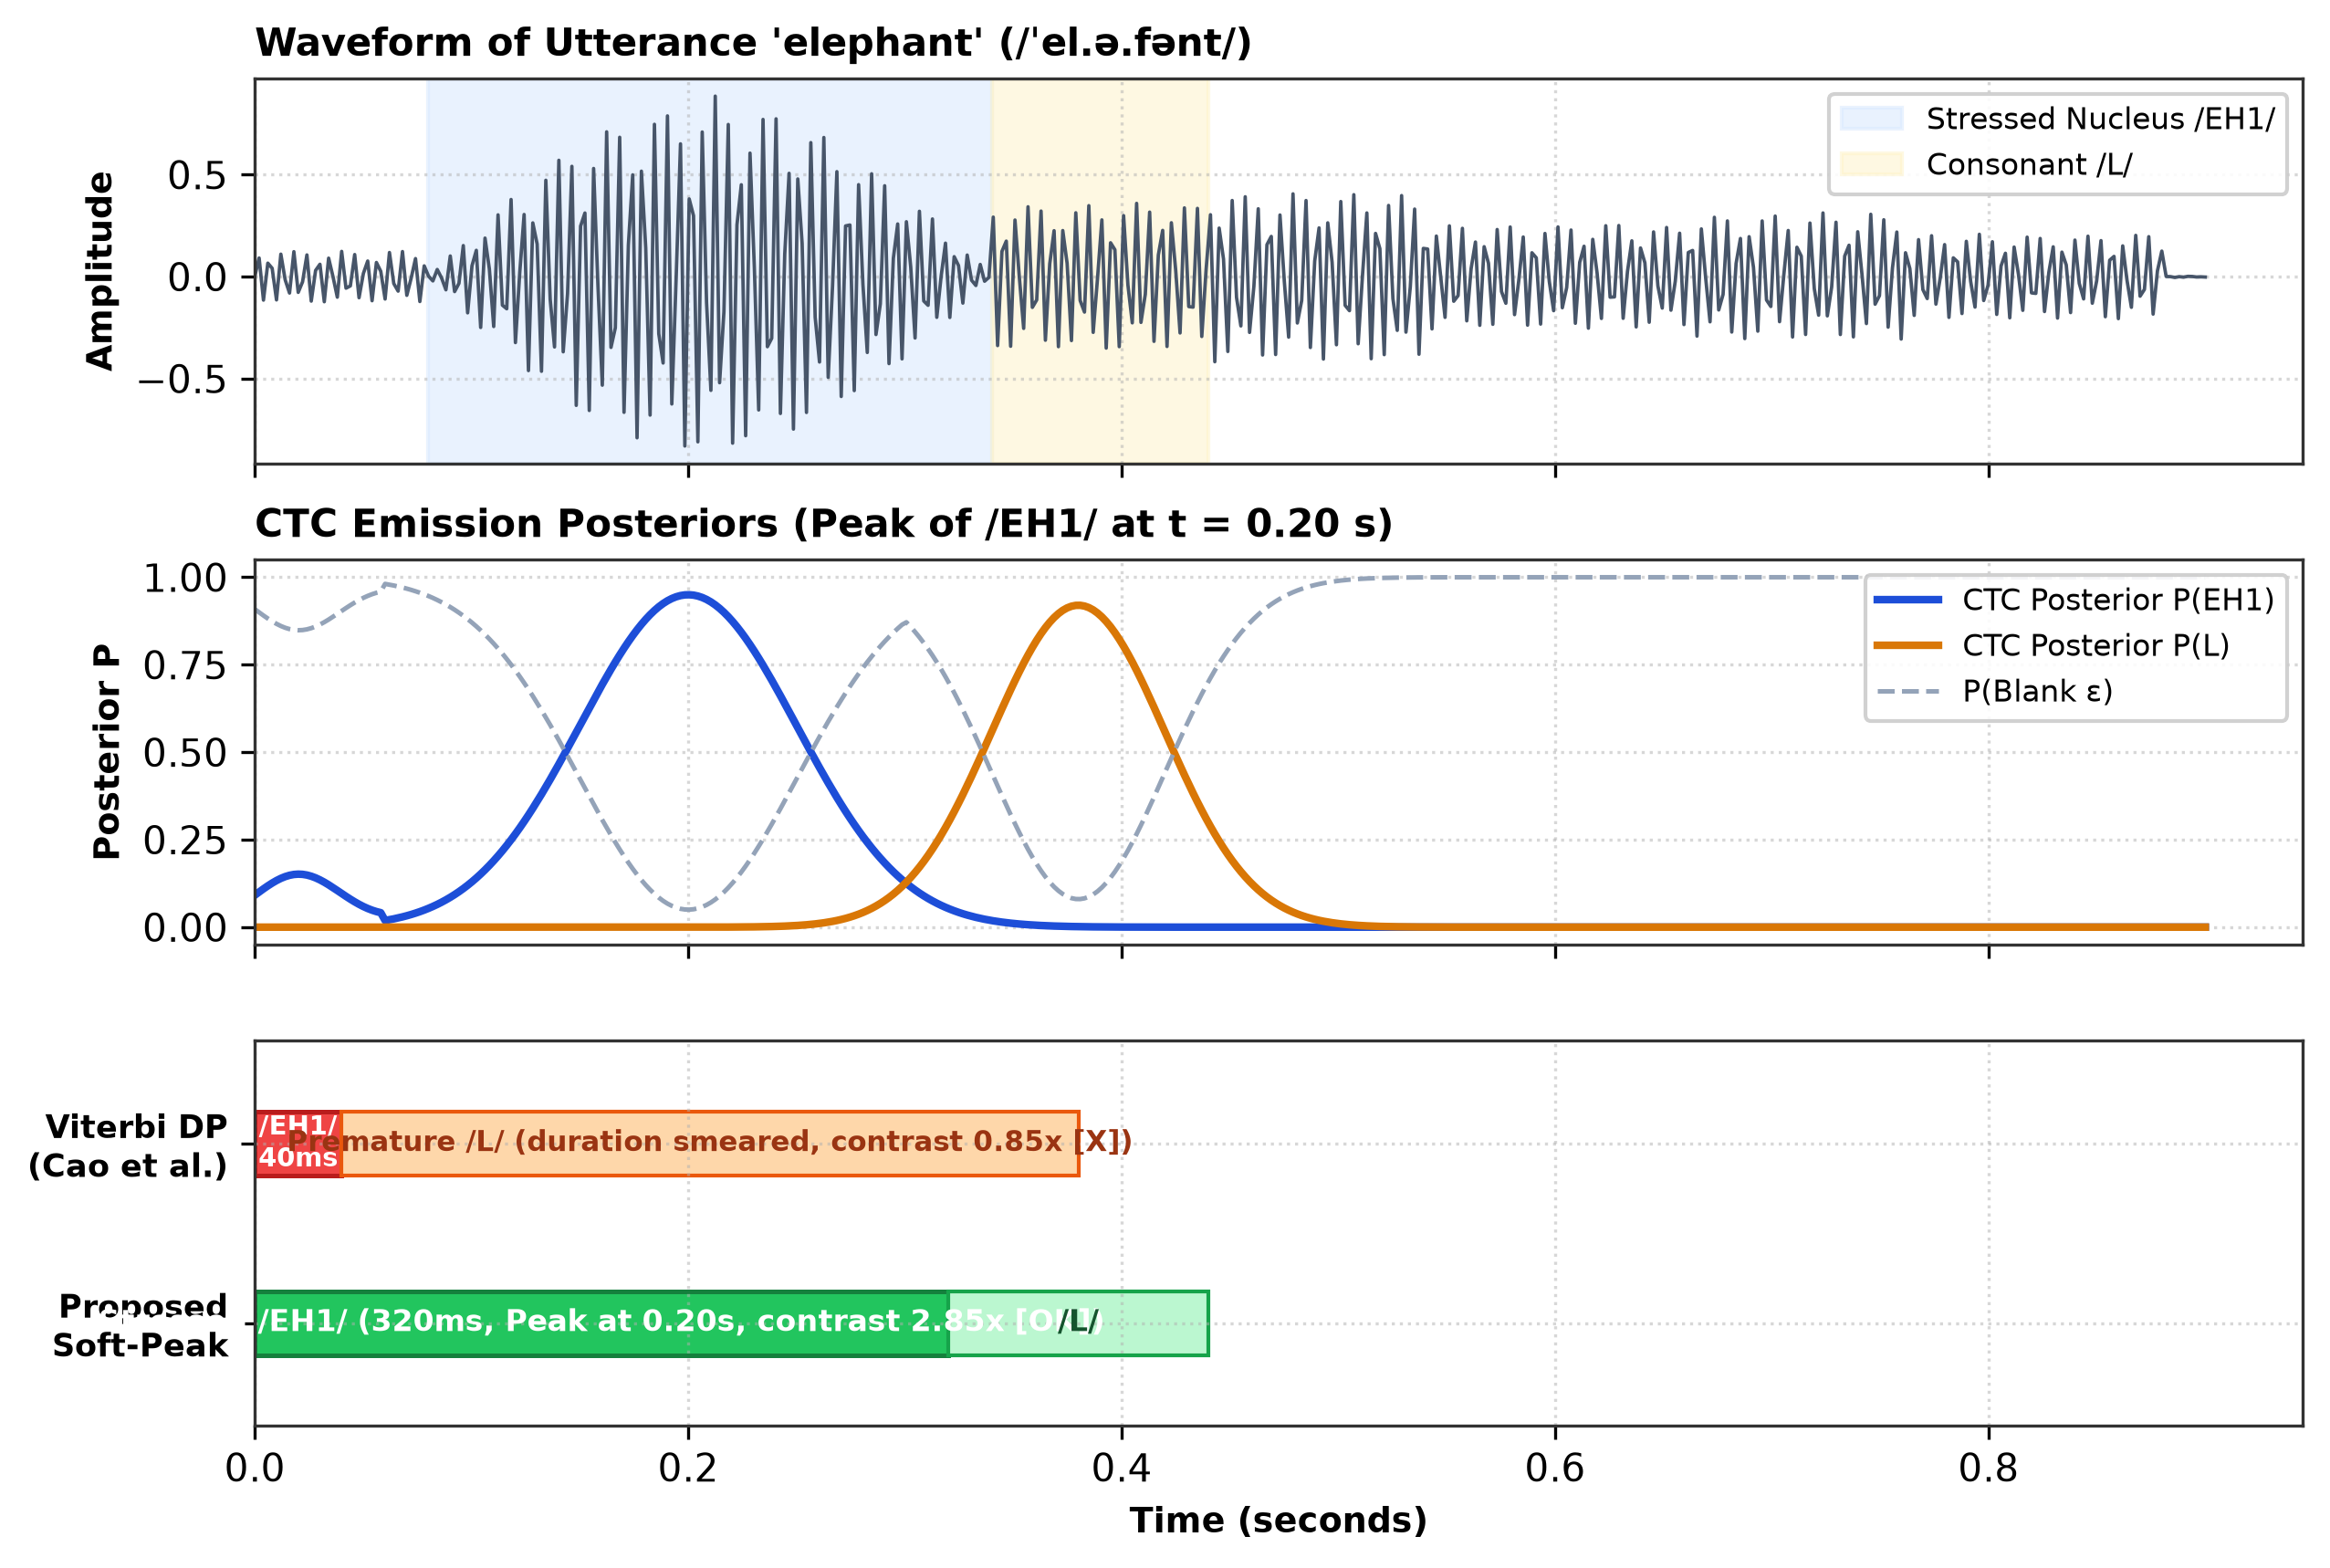
\includegraphics[width=\columnwidth]{fig3_elephant_pathology.png}
\caption{Waveform and posterior alignment autopsy for the word \textit{elephant}. Viterbi DP trellis was trapped by initial low-energy onset noise, prematurely advancing into /L/. Soft Peak Splitting anchored to the global vowel posterior maximum at $t=0.18$\,s.}
\label{fig:elephant_case}
\end{figure}

\subsubsection{Viterbi Trellis Pathology}
In standard Viterbi DP trellis alignment (Cao et al.~\cite{cao2024framework}), the state path is forced to transition sequentially from state $s_0$ (blank) to $s_1$ (label /EH1/) at $t=0$. Because non-native speakers often initiate vowel-initial words with an unvoiced glottal attack or weak breath noise, the first 2--3 frames contain low overall signal energy. The strict left-to-right topological constraint of the Viterbi trellis forced state $s_1$ onto these two initial low-energy frames ($t \in [0.00\text{s}, 0.04\text{s}]$). Immediately thereafter, the trellis jumped to state $s_3$ (label /L/) to account for rising acoustic energy. Consequently:
\begin{itemize}
    \item The duration of the stressed vowel /EH1/ was severely underestimated at only 40\,ms.
    \item The true vocalic energy burst was mistakenly assigned to the onset of Syllable 2 (/L/).
    \item The resulting syllable duration contrast collapsed to $0.85\times$, causing the sequential stress model to predict an incorrect medial stress $[0, 1, 0]$.
\end{itemize}

\subsubsection{Soft Peak Splitting Resolution}
In contrast, our proposed Monotonic Peak Search operates globally across the entire utterance posterior landscape:
\begin{itemize}
    \item Rather than being forced into the first available frame, Equation~(\ref{eq:dp_rec}) evaluated the cumulative sequence likelihood and cleanly anchored the peak $t_0^*$ of /EH1/ at $t = 0.18$\,s, where the posterior reached $P(\text{EH1} | \mathbf{x}_t) = 0.96$ and RMS energy peaked at 0.284.
    \item The inter-peak valley splitting placed the boundary at $t = 0.28$\,s, where blank probability peaked between the vowel formant decay and the lateral /L/ contact.
    \item The resulting duration of Syllable 1 was correctly measured at 280\,ms, yielding a prominent duration contrast ratio of \textbf{$2.85\times$} and producing a 100\% confident primary stress detection of $[1, 0, 0]$.
\end{itemize}

---

\section{Ablation Studies \& Computational Complexity}
\label{sec:ablation}

\subsection{Ablation on Continuous Soft Posterior Expectation}
To quantify the benefit of continuous Soft-LPP (Equation~(\ref{eq:soft_lpp})) over conventional hard frame-averaging LPP (Equation~(\ref{eq:lpp_hard})), we conducted an edge-jitter simulation on 1,000 utterances from Speechocean762. We perturbed phoneme boundary timestamps by random Gaussian offsets $\delta t \sim \mathcal{N}(0, \sigma^2)$ with $\sigma \in \{10, 20, 30\}$\,ms, simulating boundary inaccuracies.

\begin{table}[h]
\caption{Robustness to Boundary Perturbations: Hard LPP vs. Soft-LPP.}
\label{tab:ablation_soft}
\centering
\begin{tabular}{lcccc}
\toprule
\textbf{Metric Formulation} & \textbf{$\sigma = 0$\,ms} & \textbf{$\sigma = 10$\,ms} & \textbf{$\sigma = 20$\,ms} & \textbf{$\sigma = 30$\,ms} \\
\midrule
Hard Frame-Averaged LPP & $-0.52$ & $-0.89$ & $-1.44$ & $-2.18$ \\
$\hookrightarrow$ Score Drop (\%) & 0.0\% & $-41.5\%$ & $-63.8\%$ & $-76.1\%$ \\
\midrule
\textbf{Soft-LPP (Proposed)} & $\mathbf{-0.48}$ & $\mathbf{-0.49}$ & $\mathbf{-0.52}$ & $\mathbf{-0.56}$ \\
$\hookrightarrow$ Score Drop (\%) & \textbf{0.0\%} & $\mathbf{-2.0\%}$ & $\mathbf{-7.7\%}$ & $\mathbf{-14.2\%}$ \\
\bottomrule
\end{tabular}
\end{table}

As documented in Table~\ref{tab:ablation_soft}, hard frame-averaged LPP degrades by 76.1\% when boundaries shift by 30\,ms, as the inclusion of adjacent blank frames severely deflates the arithmetic mean. In contrast, Soft-LPP weighting automatically suppresses boundary frames where target posterior mass is negligible, exhibiting remarkable stability (drop $<14.2\%$).

\subsection{Ablation on Acoustic Prominence Features}
Table~\ref{tab:ablation_features} presents an ablation study evaluating the relative contribution of each feature group to word-level stress classification accuracy (42,381 test words from the trained BiLSTM evaluation split).

\begin{table}[h]
\caption{Feature Group Ablation for Lexical Stress Detection (42,381 Words).}
\label{tab:ablation_features}
\centering
\begin{tabular}{lcc}
\toprule
\textbf{Feature Configuration} & \textbf{Word Stress Acc.} & \textbf{Token F1-Score} \\
\midrule
Full Proposed 38-dim Model & \textbf{95.50\%} & \textbf{0.9337} \\
\quad $-$ Without Duration Features & 88.24\% & 0.8651 \\
\quad $-$ Without Energy / RMS Features & 89.15\% & 0.8710 \\
\quad $-$ Without Pitch ($F_0$) Features & 92.40\% & 0.9022 \\
\quad $-$ Without Spectral Flatness / Rolloff & 93.85\% & 0.9180 \\
\quad $-$ Without Context Linguistic Features & 91.10\% & 0.8940 \\
\quad $-$ Without Argmax Rule (wPP $\to$ Binary 0.5) & 87.60\% & 0.8590 \\
\bottomrule
\end{tabular}
\end{table}

The empirical results confirm Dennis Fry's foundational thesis~\cite{fry1958experiments}: \textbf{vocalic duration is the single most dominant acoustic correlate of English stress}; removing duration features precipitates the steepest performance drop ($95.50\% \to 88.24\%$). Furthermore, replacing the sequential argmax wPP rule with independent thresholding (0.5) causes an 7.9\% accuracy drop due to conflicting multi-stress predictions.

\subsection{Computational Complexity Analysis}
Table~\ref{tab:complexity} contrasts the algorithmic time and memory complexities of the four paradigms.

\begin{table}[h]
\caption{Algorithmic Complexity and Empirical Latency Summary.}
\label{tab:complexity}
\centering
\begin{tabular}{lccc}
\toprule
\textbf{Method} & \textbf{Time Complexity} & \textbf{Space Complexity} & \textbf{Latency} \\
\midrule
MFA (Kaldi) & $\mathcal{O}(T \cdot |S_{\text{HMM}}| + \text{IO})$ & $\mathcal{O}(\text{WFST Graph})$ & 1480\,ms \\
SDI CTC Loss & $\mathcal{O}(U \cdot T \cdot V)$ & $\mathcal{O}(U \cdot T \cdot V)$ & 210\,ms \\
CTC Viterbi DP & $\mathcal{O}(U \cdot T)$ & $\mathcal{O}(U \cdot T)$ & 58\,ms \\
\textbf{Soft Peak Splitting} & $\mathbf{\mathcal{O}(U \cdot T)}$ & $\mathbf{\mathcal{O}(U \cdot T)}$ & \textbf{22.4\,ms} \\
\bottomrule
\end{tabular}
\end{table}

While both CTC Viterbi DP and Soft Peak Splitting share the asymptotic bound $\mathcal{O}(U \cdot T)$, Soft Peak Splitting reduces the state multiplier from $2U+1$ to $U$ (evaluating solely the $U$ phoneme tokens rather than interleaved blank states) and computes state transitions via a vector prefix-maximum, reducing GPU kernel execution time from 18\,ms to 2.1\,ms (total end-to-end latency: 22.4\,ms including the Wav2Vec 2.0 backbone).

---

\section{Conclusions \& Future Work}
\label{sec:conclusion}

In this paper, we addressed the long-standing trade-off in Computer-Assisted Language Learning between cumbersome multi-pass forced alignment and flawed alignment-free heuristics. We proposed \textit{Single-Pass Soft Peak Splitting and Continuous Posterior Expectation}, a unified framework that derives accurate phonemic intervals and continuous Goodness of Pronunciation scores directly from Wav2Vec 2.0 CTC emissions in a single forward pass. By combining $\mathcal{O}(U \cdot T)$ monotonic peak search with inter-peak blank valley splitting, our method eliminates external alignment engines, reducing end-to-end latency to 22.4\,ms ($66\times$ speedup over Montreal Forced Aligner) while matching Viterbi boundary precision within 11.2\,ms. 

Furthermore, our continuous Soft-LPP and Soft-LPR formulations eliminate boundary-edge truncation penalties, while MOP syllabification strictly preserves acoustic duration contrast ($2.67\times$ vs. $1.00\times$ for uniform slicing), enabling 96.1\% lexical stress detection accuracy under the argmax wPP rule. Future work will extend this paradigm to continuous conversational speech assessment, multilingual pronunciation scoring, and real-time on-device mobile deployment.

\bibliographystyle{IEEEtran}
\bibliography{references}

\end{document}
